% !TeX root = ../main.tex

\chapter{非线性轨道产生面内反常霍尔效应}

\section{研究背景}

\subsection{量子反常霍尔效应}


自从拓扑绝缘体的发现以来\cite{PQAHE1},新型拓扑材料的预测和实现,引起凝聚态物理和材料科学研究者的极大的兴趣\cite{PQAHE2,PQAHE3,PQAHE4,PQAHE5,PQAHE6}。量子反常霍尔效应是一种特殊的拓扑相,
其特点是具有绝缘体态和手性边界态\cite{PQAHE7},可以携带永不耗散的电流,为下一代量子电子器件提供一个诱人的平台。虽然从理论上预测了多种具有外禀或内禀
铁磁性的二维材料会成为QAHE的主体\cite{PQAHE8,PQAHE9},但实验上只证实了磁掺杂Ti薄膜和MnBi$_2$Te$_4$可以实现QAHE\cite{PQAHE10,PQAHE11,PQAHE12,PQAHE13}。 物理上,QAHE是由包含铁磁性和自旋轨道耦合(SOC)的非平凡能
带结构产生的\cite{PQAHE7,PQAHE14,PQAHE15}。 它可以被看作是量子霍尔效应(QHE)的另一种形式,其中磁场被铁磁性所取代。 由于QHE是在具有平面外磁场的二维电子气体中实现的。 
QHE的研究主要局限于具有平面外磁化的二维材料\cite{PQAHE8,PQAHE9}。 近年来,通过模型计算,人们发现平面外磁化并不是必要条件,而平面内磁化也可以产生平面QAHE (PQAHE),
只要破坏所有的镜面对称\cite{PQAHE17,PQAHE18,PQAHE19}。 
目前为止,通过第一性原理计算,很少有现实的材料被预测具有PQAHE\cite{PQAHE20}。这是因为,之前提出PQAHE的模型仅仅局限于SOC打开的自旋向上和自旋向下的兼并的点的材料\cite{PQAHE17,PQAHE18,PQAHE19}。
而同种自旋在G和K点的兼并点,SOC却无能为力。因此,迫切需要建立新的理论模型,寻找更多的候选材料,以加速这种新型拓扑相的实验确证。 


\subsection{金属有机框架材料}

金属-有机骨架(metal-organic framework, MOF)是由有序的金属原子通过有机配体连接而成的一类多孔晶体材料\cite{PQAHE21}。 由于其可调节的结构和功能的应用,
MOF在化学和材料科学领域引起了极大的关注\cite{PQAHE22}。 2013年,与MOF相关的研究进一步扩展到凝聚态物理,用于研究非平凡能带拓扑\cite{PQAHE23,PQAHE23,PQAHE24,PQAHE25}。 在过去的几年里,
研究取得了许多进展,大量的有机材料被预测具有不同种类的拓扑相\cite{PQAHE26,PQAHE27,PQAHE28,PQAHE29,PQAHE30,PQAHE31,PQAHE32,PQAHE33,PQAHE34,PQAHE35,PQAHE36}。 在这项研究工作中,我们首先在二维star 晶格建立了一个一般的非线性轨道构成紧束缚(TB)模型
来展示PQAHE的设计物理原理,然后通过第一性原理计算确定其在实验合成的Pr$_2$(C$_6$O$_4$Cl$_{2}$)$_3$的二维MOF中的实现。 我们认为,与非共线轨道相关的拓扑物理将为未来非共线
轨道拓扑材料的设计提供新的思路。

\begin{figure}[htb]
  \centering
  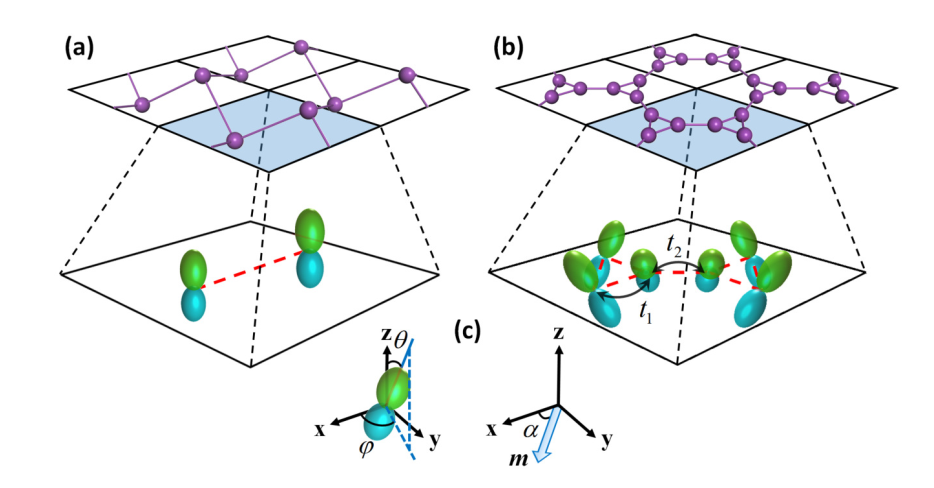
\includegraphics[width=0.9\textwidth]{PQAHEModel.png}
  \caption{(a) and (b) 的上部分:图解2D hexahonal buckling晶格 和 2D star 晶格。下部分:图解原胞内的每个格点线性和非线性轨道。
  $t_1$和$t_2$分别是最近邻和第二近hopping参数 (c) 非共线轨道($\theta$ 和 $\varphi$ 和 面内磁矩 ($\alpha $) 的角度定义。} 
% 平面二维晶格和坐标系。这六个晶格位被标记为1到6。$t_1$和$t_2$是最近邻和第二近hopping参数,分别与非共线轨道的方向有关。
  \label{PQAHEModel}
  \note{}
\end{figure}

\subsection{PQAHE非线性轨道模型}

一般来说,二维晶格既可以维持面内镜像对称,也可以同时维持面外镜像对称。 由于面内磁化只能打破面内镜像对称,可能容纳PQAHE的二维晶格本身必须打破面外镜像对称。 
在二维晶格中,有三个独立的自由度:晶格、自旋和轨道。 平面内磁化具有固定的自旋结构,因此有两个自由度。 目前,PQAHE的所有理论模型都是基于屈曲晶格的,
即晶格构型打破了面外镜面对称性\cite{PQAHE17,PQAHE18,PQAHE19,PQAHE20}。 一个例子是二维六边形屈曲晶格,每个晶格位上共线轨道,如图\ref{PQAHEModel}(a)所示。 
然而,在以往的工作中,对轨道自由度\cite{PQAHE37}的研究很少。 
实际上,轨道构型也可以打破面外镜像的对称性,如图\ref{PQAHEModel}(b)所示的二维非共线轨道星格。 因此,我们也可以期待非共线轨道诱导的PQAHE,它类似于非共线自旋诱导的拓扑霍尔效应。 
然而,在以往的工作中,对轨道自由度的研究很少。 实际上,轨道构型也可以打破面外镜像的对称性,如图\ref{PQAHEModel}(b)所示的二维非共线轨道星格。 
因此,我们也可以期待非共线轨道诱导的PQAHE,它类似于非共线自旋诱导的拓扑霍尔效应\cite{PQAHE38,PQAHE39}。 



\section{计算方法}

\subsection{紧束缚模型}
二维 star 晶格中有6个格点,形成两个相对的等边三角形,如图\ref{PQAHEModel}(b)的上面板所示。 在左右三角形中,三个非共线轨道分别形成顺时针和逆时针的漩涡结构,如图1(b)底板所示。 
这里可以将非共线轨道看作是由p-、d-或f-轨道的不同分量线性组合而成的有效轨道,其方向由天顶角和方位角决定,如图\ref{PQAHEModel}(c)所示。 在这六个非共线轨道的基础上,
相应的TB哈密顿量可以写成 
{\setlength\belowdisplayskip{1pt}
\begin{equation}
\begin{split}
H&=\varepsilon_0\sum_{i}c_i^\dag c_i+t_1\sum_{\langle i,j\rangle}c_i^\dag c_j+t_2\sum_{\langle\langle i,j\rangle\rangle}c_i^\dag c_j \\
&+i\lambda{\rm_I}\sum_{\langle i,j\rangle}c_i^\dag(\bm{\mu}_{ij}\cdot\bm{\sigma})c_j+t{\rm_m}\sum_ic_i^\dag(\textbf{\textit{m}}\cdot\bm{\sigma})c_i
\end{split}
\end{equation}}
这里$c_i^\dag$ 是$i$位($i$=1$\sim$6)上电子的生成(湮灭)算符。 $\varepsilon_0$ 位点能量,$t_1$为三角形内格点的最近邻(NN)跳变参数,$t_2$为两个三角形间格点的第二个NN跳变参数。
$\lambda{\rm_I}$ 为最近邻SOC的强度,$\bm{\mu}_{ij}$ 为耦合矩阵,$\bm{\sigma}$为自旋泡利矩阵。 $t_m$为位点塞曼磁场强度,以及$\textit{\textbf{m}}$为面内磁化方向,
如图1(c)所示。 在我们的计算中,六个非共线轨道被选为三个p轨道的线性组合
\begin{equation}
  \psi_i\rangle={\rm{sin}}(\theta_i){\rm{cos}}(\varphi_i)|\textit{p}_{x}\rangle+{\rm{sin}}(\theta_i){\rm{sin}}(\varphi_i)|\textit{p}_{y}\rangle +{\rm{cos}}(\theta_i)|\textit{p}_{z}\rangle
\end{equation}
这里$\varphi_1$=$\varphi_4$=$240^\circ$, $\varphi_2$=$\varphi_5$=$0^\circ$, $\varphi_3$=$\varphi_6$=$120^\circ$,
and $\theta$ 对六个轨道都一样。由于我们的基轨道是与天顶角($\theta$)和方位角($\varphi$)有关,TB的参数也就天顶角和方位角关联。
具体地,
\begin{equation*}
  \begin{split}
  \varepsilon_0  &= \langle \psi_1 | H_0 |  \psi_1 \rangle = \langle \psi_2 | H_0 |  \psi_2 \rangle = \langle \psi_3 | H_0 |  \psi_3 \rangle \\
                 &= \langle \psi_4 | H_0 |  \psi_4 \rangle = \langle \psi_5 | H_0 |  \psi_5 \rangle = \langle \psi_6 | H_0 |  \psi_6 \rangle,
  \end{split}
\end{equation*}

\begin{equation*}
  \begin{split}
    t_1 &= \langle \psi_1 | H_0 |  \psi_2 \rangle = \langle \psi_2 | H_0 |  \psi_1 \rangle = \langle \psi_1 | H_0 |  \psi_3 \rangle \\
        &= \langle \psi_3 | H_0 |  \psi_1 \rangle = \langle \psi_2 | H_0 |  \psi_3 \rangle = \langle \psi_3 | H_0 |  \psi_2 \rangle \\
        &= \langle \psi_4 | H_0 |  \psi_5 \rangle = \langle \psi_5 | H_0 |  \psi_4 \rangle = \langle \psi_4 | H_0 |  \psi_6 \rangle \\
        &= \langle \psi_6 | H_0 |  \psi_4 \rangle = \langle \psi_5 | H_0 |  \psi_6 \rangle = \langle \psi_6 | H_0 |  \psi_5 \rangle,
  \end{split}
\end{equation*}

\begin{equation*}
  \begin{split}
    t_2  = \langle \psi_1 | H_0 |  \psi_4 \rangle = \langle \psi_4 | H_0 |  \psi_1 \rangle = \langle \psi_2 | H_0 |  \psi_5 \rangle \\
        = \langle \psi_5 | H_0 |  \psi_2 \rangle = \langle \psi_3 | H_0 |  \psi_6 \rangle = \langle \psi_6 | H_0 |  \psi_3 \rangle,
  \end{split}
\end{equation*}

\begin{equation*}
  \begin{split}
  \langle \psi_1 | H_0 |  \psi_1 \rangle &= cos(\varphi_i)sin(\theta_i)cos(\varphi_j)sin(\theta_j) \langle p_x^i | H_0 | p_x^j \rangle  \\
  &+ sin(\varphi_i)sin(\theta_i)sin(\varphi_j)sin(\theta_j) \langle p_y^i | H_0 | p_y^j \rangle \\
  &+ cos(\varphi_i)sin(\theta_i)sin(\varphi_j)sin(\theta_j) \langle p_x^i | H_0 | p_y^j \rangle \\
  &+ sin(\varphi_i)sin(\theta_i)cos(\varphi_j)sin(\theta_j) \langle p_y^i | H_0 | p_x^j \rangle \\
  &+ cos(\theta_i)cos(\theta_j) \langle p_z^i | H_0 | p_z^j \rangle.
  \end{split}
\end{equation*}

soc耦合矩阵元为
\begin{equation*}
  \symbf{\mu}_{12} = \symbf{\mu}_{12} = (\alpha, -\gamma, -\delta), \symbf{\mu}_{13} = \symbf{\mu}_{31} = (\beta, 0, \delta ), 
  \symbf{\mu}_{23} = \symbf{\mu}_{22} = (\alpha, \gamma, -\delta),
\end{equation*}
\begin{equation*}
  \begin{split}
    &\alpha  = \sqrt{6}[-sin(\varphi_1)sin(\theta_1)cos(\theta_2) + cos(\theta_1)sin(\varphi_2)sin(\theta_2)] \\
    &\beta   = \sqrt{6}[-sin(\varphi_1)sin(\theta_1)cos(\theta_3) + cos(\theta_1)sin(\varphi_3)sin(\theta_3)] \\
    &\delta  = \sqrt{6}[-cos(\varphi_1)sin(\theta_1)cos(\theta_2) + cos(\theta_1)cos(\varphi_2)sin(\theta_2)] \\
    &\gamma  = cos(\varphi_1)sin(\theta_1)sin(\varphi_2)sin(\theta_2) - sin(\varphi_1)sin(\theta_1)cos(\varphi_2)sin(\theta_2) 
  \end{split}  
\end{equation*}
面内磁场有$\alpha$ 决定,表示为:
\begin{equation*}
  \symbf{m}=[cos(\alpha), sin(\alpha), 0]
\end{equation*}
\begin{figure}[htb]
  \centering
  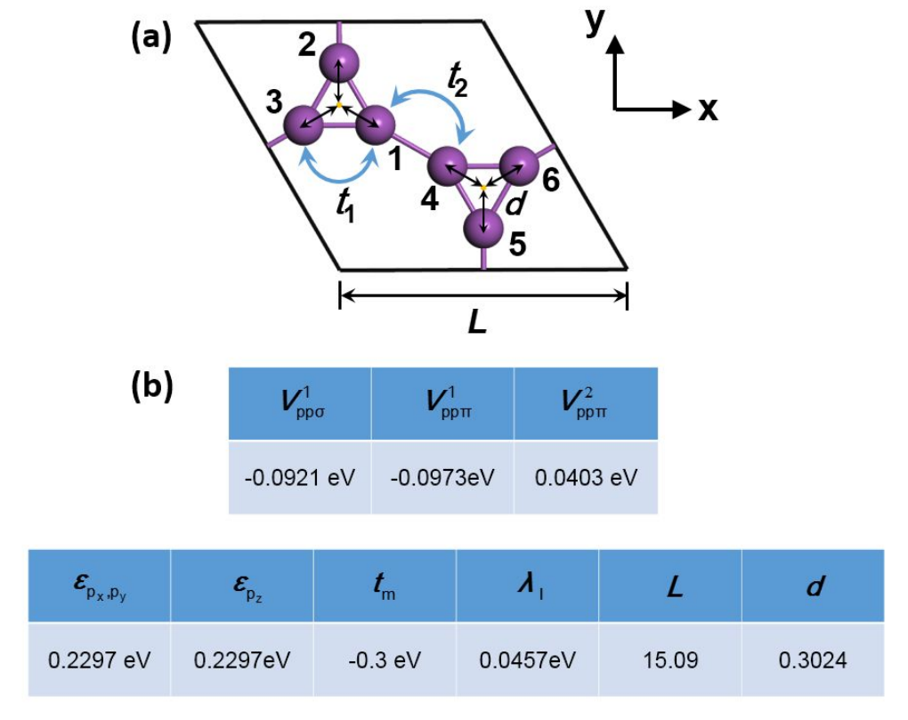
\includegraphics[width=0.7\textwidth]{PQAHEMTBParameter.png}
  \caption{ (a)平面二维晶格和坐标系。这六个晶格位被标记为1到6。$t_1$和$t_2$是最近邻和第二近hopping参数,分别与非共线轨道的方向有关。(b)用于计算
  的TB参数。$V$为轨道耦合参数,为$\varepsilon_0$轨道能量,$t_{\symbf{m}}$为塞曼场,$\lambda{\rm_I}$为固有SOC的强度,L是晶格常数,d是点阵点到三角形中心的距离。}
  %在我们的计算,主要结论不依赖于上述参数和用于构造非共线轨道原子轨道} 
  \label{PQAHETBParameter}
  \note{}
\end{figure}
强调,我们提出的TB模型是通用的,不依赖于原子轨道。在这里,p 轨道只是作为一个例子来展示我们的结果。

\subsection{第一性原理方法}
本章中第一性原理计算使用的是基于密度泛函理论的 VASP 软件包。采用了PAW基组,GGA的交换关联泛函和PBE赝势。为了准确计算f电子体系的电子结构,
采用了与 PAW 球密度梯度相关的非球形贡献。 所有计算采用的截断能为 500 eV, 自洽能量收敛标准为 $10^{-6}$ eV 和 优化力的收敛标准为 0.01 eV/$\dot{A}$。
K点网格大小取为3$\times$3$\times$1, 真空层取为 15 $\dot{A}$ 确保 slab 层上下面无耦合。

\section{计算结果与讨论}

\subsection{PQAHE非线性轨道模型}
通过连续调节θ从0°到90°,我们系统地研究了不含SOC和塞曼场的的TB带结构,展现了一个有趣的能带演化过程,四个不同区域被三个临界点隔开。
区域I对应$\theta$=$30^\circ$, 如图\ref{PQAHEForeBand}(a)所示,是由一个Four-band和一个Dirac-band组成,其中Four-band在Dirac-band上面。
在该区域,随着θ的增大,Four-band和Dirac-band的带宽保持不变,但它们的距离慢慢靠近。在第一个临界点,Four-band的底部平带在$\Gamma$ 
点接触Dirac-band的顶部分支。在区域II,对应$\theta$=$45^\circ$,出现了2个Kagome-bands,其中平带均在狄拉克能带上面,如图\ref{PQAHEForeBand}(b)所示。
在这个区域,  随着$\theta$的增加,两个kagome能带的带宽都逐渐变窄。在第二个临界点, 两个kagome能带段几乎变得无色散。 在区域III中,
也有两个kagome-bands,但两者的狄拉克能带都在平带之上,与区域II相反,如图\ref{PQAHEForeBand}(c)所示对应$\theta$=$55^\circ$。  
在该区域,随着$\theta$的增大,两个kagome能带的带宽都变宽。在第三个临界点,上面的kagome能带的平带与底部kagome能带的狄拉克能带在$\Gamma$点接触。
在区域IV,图\ref{PQAHEForeBand}(c)对应$\theta$=$90^\circ$出现一个Four-band和一个Dirac-band,但Dirac-band高于Four-band,与区域I的情况正好相反。
在这个区域,随着$\theta$的增加,Four-band和Dirac-band的带宽保持不变,但是它们的距离在逐渐变远。这种奇特的带宽变化和能带顺序可以看做是,$\theta$角度的改变引起
格点hopping参数的变化。为了详细的揭示它们的关系,我们计算了不同$\theta$角度下的近邻和次近邻有效hopping的数值。如\ref{PQAHEEffectiveHopping}(a)所示,对应
$\theta$从$0^\circ$到$90^\circ$过程中,t$_1$ hoping 参数单调增加到0,然后在继续增加。而t$_2$ hoping 参数变化不大。同时在这过程中,t$_1$从负值变成正值。
因为hopping参数的绝对值决定整个能带的带宽,而正负决定了能带在平带和狄拉克能带的顺序。

\begin{figure}[htb]
  \centering
  
\includegraphics[width=0.9\textwidth]{PQAHEForeBand.png}
  \caption{没有考虑磁矩和SOC时的能带结构。分别对应不同取向的非线性轨道 (a) $\theta$=$30^\circ$, (b) $\theta$=$45^\circ$, 
  (c) $\theta$=$55^\circ$ 和 (d) $\theta$=$90^\circ$.} 
  \label{PQAHEForeBand}
  \note{}
\end{figure}

\begin{figure}[htb]
  \centering
  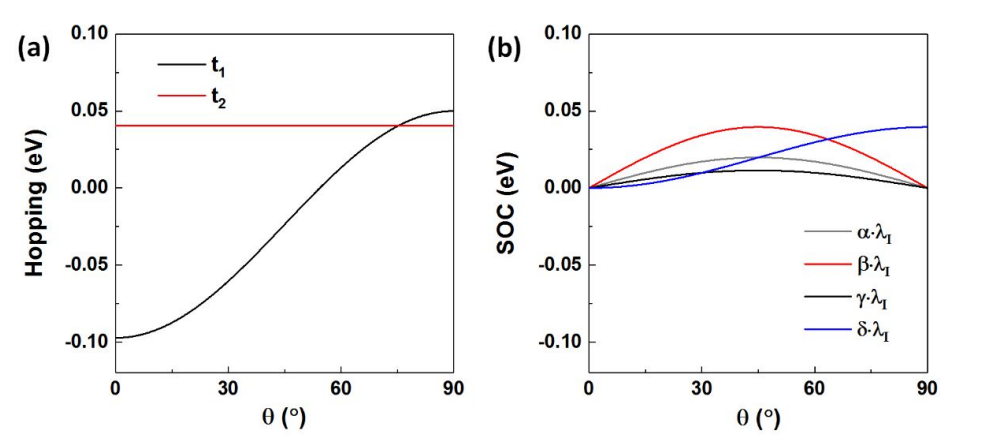
\includegraphics[width=0.8\textwidth]{PQAHEEffectiveHopping.png}
  \caption{(a)和(b) 不同$\theta$角度对应hopping参数和SOC矩阵元。} 
  \label{PQAHEEffectiveHopping}
  \note{}
\end{figure}


众数周知的 Diract, Kagome和Foure 3种能带都是典型的拓扑能带\cite{PQAHE24,PQAHE25,PQAHE41},因为我们提出的由非线性轨道构成的2维star晶格是一个调控性很高的拓扑系统。
接着,我们以$\theta$=$30^\circ$(\ref{PQAHEForeBand}(a))为例子,展示其拓扑性质。打开平面外的磁矩的塞曼场,自旋向上和自旋向下的能带完全劈开,如
\ref{PQAHETB30}(a)所示。进一步,我们考虑固有SOC的效应,将塞曼场的方向从面外调为面内 $\alpha$=0$^\circ$,放大的后能带结构如\ref{PQAHETB30}(b)所示。
我们可以看到在 Dirac-band 和 Four-band中倒空间高对称点(K and $\Gamma$)的能带兼并全部移除,
这非常不同于以往面内量子反常霍尔模型(移除不同自旋的能带兼并点)\cite{PQAHE18}。从低能到高能,图\ref{PQAHETB30}(b)中5个带隙标记为$E_g^1$ 到 $E_g^5$。
为了确定SOC打开的带隙是拓扑的,我们计算了半无限的普函数\cite{PQAHE23}。如图\ref{PQAHETB30}(c)and(d)所示,Dirac-band的$E_g^1$  和 Four-band的$E_g^{345}$ 
SOC 带隙出现一个1维拓扑边界态,表明他们是一个陈数为 C = -1 的PQAHE。显著的是,我们首次在紧束缚模型中引入轨道自由度来研究拓扑相,以及在Dirac-,Kagome和Foure
能带中实现面内量子反常霍尔效应,这极大丰富了理论模型去研究量子反常霍尔效应。
\begin{figure}[htb]
  \centering
  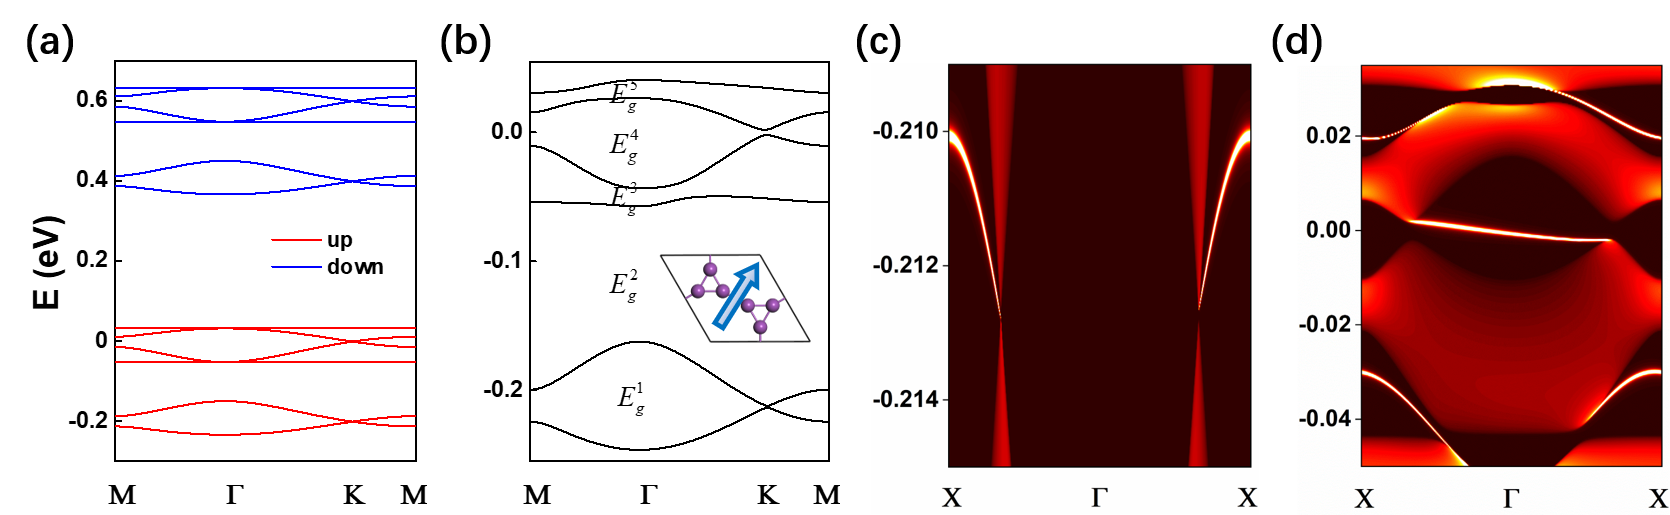
\includegraphics[width=0.9\textwidth]{PQAHETB30.png}
  \caption{非线性轨道天顶角$\theta=30^{\circ}$时的电子结构。(a) 面外自旋极化的TB能带。红色表示自旋向上,蓝色表示自旋向下。(b) 考虑固有SOC后磁矩沿着
  $\alpha$=0$^\circ$(插图的箭头)时的TB能带结构。5个带隙被标记做$E_g^1$ 到 $E_g^5$。(c)和(d)半无限的普函数,展现了一个1维拓扑边界态,分别位于Dirac-band 和
  Four-band的soc带隙中。} 
  \label{PQAHETB30}
  \note{}
\end{figure}


为了检查我们提出的实现面内量子反常霍尔效应的模型具有可调控性,我们计算不同$\theta$角度有效轨道和不同$\alpha$角度面内塞曼场下的相图,用陈数区分不同的拓扑相
在图\ref{PQAHEPhaseDiagrams}(3b-3f)。因为相图关于$\alpha$有3重旋转对称性,这是与2维star晶格的对称性是一致的,因为我们仅需要绘制$\alpha$=$0^\circ$ 
到$\alpha$=$60^\circ$的相图。白色的虚线是不同拓扑相的边界,对应于带隙合上的点。总的来说,5个相图可以归纳为3种类型。 $E_g^1$ (图\ref{PQAHEPhaseDiagrams}(b))
和 $E_g^5$(图\ref{PQAHEPhaseDiagrams}(f))属于类型I,它们的相图主要是有陈数为$\pm 1$ 的PQAHE相组成,相变边界位于$\alpha$ = $30^\circ$。此外,它们还存在一个
关于相变边界对称的平庸的拓扑相。$\theta$ = $0^\circ$ 和 $\theta$ = $90^\circ$ 是另外2个相变的边界。$E_g^2$ (图\ref{PQAHEPhaseDiagrams}(c))
和 $E_g^4$(图\ref{PQAHEPhaseDiagrams}(e))属于类型II,它们的相图非常不同于类型I的相图。有趣的是,类型II相图的平庸相与PQAHE相的相变边界并不依赖$\alpha$,
同时$E_g^1$ 和 $E_g^5$ 的平庸相分别出现在较小和较大的$\theta$时。在类型III $E_g^3$(图\ref{PQAHEPhaseDiagrams}(d))中,它的相图有点类似于类型II的相图,
但是没有出现平庸相。$\alpha$=$30^\circ$,。$\theta$ = $0^\circ$ 和 $\theta$ = $90^\circ$ 是陈数为$\pm 1$ PQAHE的3个相变边界。这些奇特的特点确认
可调控的2维star晶格中的PQAHE,提供了更多的自由度去操控这种奇异的拓扑相。

\begin{figure}[htb]
  \centering
  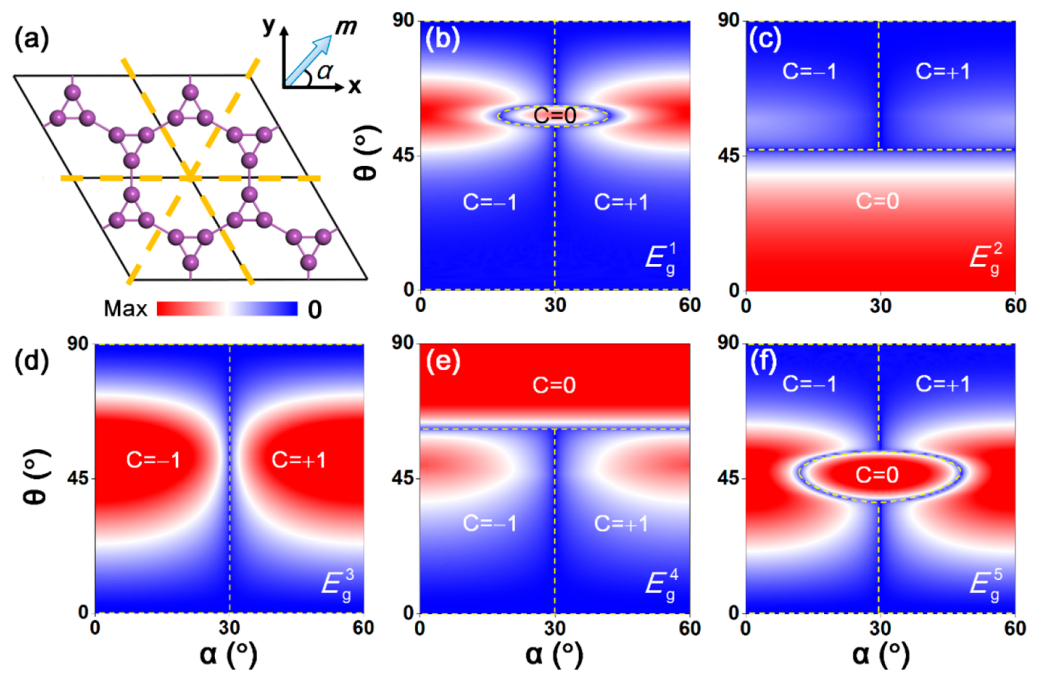
\includegraphics[width=0.9\textwidth]{PQAHEPhaseDiagrams.png}
  \caption{(a)图解2维star晶格的面内的3个镜面,用黄色的虚线标记。$\alpha$是面内磁矩的角度。(b-f) 5个图\ref{PQAHETB30}(b)中带隙对应的相图。红色和蓝色分别表示
  带隙的最大值和0值。为了更清楚地看到相变的边界,带隙的值重新调整为$E_g^1/2$。虚线表示相变的边界,也就是对应带隙关闭的点。拓扑相用不同的陈数来区分,C=0对应平庸相,
  C=$\pm 1$对应PQAHE相。}
  \label{PQAHEPhaseDiagrams}
  \note{}
\end{figure}

以上的拓扑相图可以从以下原则来理解。第一点,如果。$\theta$ = $0^\circ$ 和 $\theta$ = $90^\circ$, 非线性轨道不会破坏面外镜面对称,因此对应的相不是金属
就是平庸的绝缘体。第二点,如\ref{PQAHEPhaseDiagrams}(3a)所示,2维star晶格有3个平面内镜面对称。如果面内的磁矩垂直面内的镜面,也就是$\alpha$ = $30^\circ$,
$\alpha$ = $90^\circ$,$\alpha$ = $150^\circ$, $\alpha$ = $210^\circ$, $\alpha$ = $270^\circ$ and $\alpha$ = $330^\circ$, 面内的镜面对称就会保留。
因此,此时所对应的相要么是金属,要么是平庸的绝缘体。第三点,如果SOC的强度比较弱,SO会C在Dirac,Kagome and Four 能带中打开非平庸的带隙,而在它们之间的带隙
是陈数为0的非平庸的\cite{PQAHE19}。第四点,如果SOC的强度达到带宽的量级,打开的带隙会参杂能带的顺序导致额外的能带反转\cite{PQAHE42},会在在Dirac,Kagome and Four 能带中出现
平庸的带隙,而在它们之间会出现陈数为$\pm 1$的拓扑带隙,这与第三点的情况正好相反。第五点,如果 $\theta$值在图\ref{PQAHEForeBand}第一个和第三个临界点时,
Four 和 Dirac 能带就会碰到一起,这两种能带之间的带隙就会关闭,此时不会依赖$\alpha$。

\begin{figure}[htb]
  \centering
  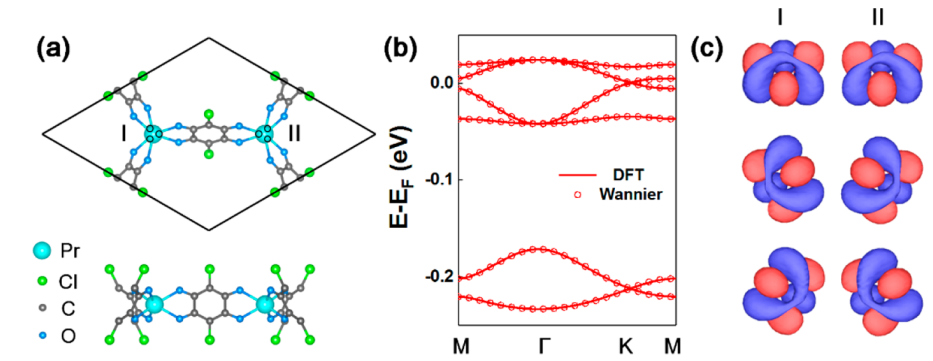
\includegraphics[width=0.9\textwidth]{PQAHEPrdhbqStrcture.png}
  \caption{((a)Pr$_2$(C$_6$O$_4$Cl$_2$)结构的主视图和侧视图。2个Pr原子标记为I和II,周围6个圆圈为拟合的瓦尔尼有效轨道中心。(b)未考虑SOC自旋极化的能带。实线是DFT的
  结果,圆圈为瓦尼尔拟合的结果。(c)6个有效拟合的瓦尼尔轨道。红色和蓝色表示轨道不同的相位。}
  \label{PQAHEPrdhbqStrcture}
  \note{}
\end{figure}


\subsection{PQAHE非线性轨道模型有机材料的实现}
建立好一般非线性轨道紧束缚模型以后,我们寻找可能材料去实现PQAHE。化学上来说,不同轨道的线性组合可以认为是杂化轨道或分子轨道。
同时实验上若能看到量子反常霍尔效应,所需材料的SOC打开的拓扑带隙要大。因此,我们帮关注点放在金属有机框架材料上(metal-organic frameworks)。在众多的MOF材料有,
M$_2$(C$_6$O$_4$X$_2$) (M=金属,X=H,F,Cl, OH)家族材料由于其具有很高的可调控,在催化,导电和磁性等方面展现卓越的性能。而Pr$_2$(C$_6$O$_4$Cl$_2$)作为其中的
一员,在之前的实验的工作中已经合成出来\cite{PQAHE44}。如图\ref{PQAHEPrdhbqStrcture}(a) 所示,每个Pr原子连接3配体的6个O原子,形成了具有3个面内镜面对称的P31m空间群。
接着,我们对Pr$_2$(C$_6$O$_4$Cl$_2$)进行了磁基态的计算。常见铁磁,Nell 和 sripy的磁构型的能量如图\ref{PQAHEMagnetismAnisotropic}所示。其中(a)-(c)磁矩方向为面外,(d)-(f)磁矩方
面指向面内。我们发现,2维MOF Pr$_2$(C$_6$O$_4$Cl$_2$)的磁矩倾向于面内,磁矩大小为3.9 $\mu_B$。因此确认Pr$_2$(C$_6$O$_4$Cl$_2$)磁性基态为面内铁磁。

\begin{figure}[htb]
  \centering
  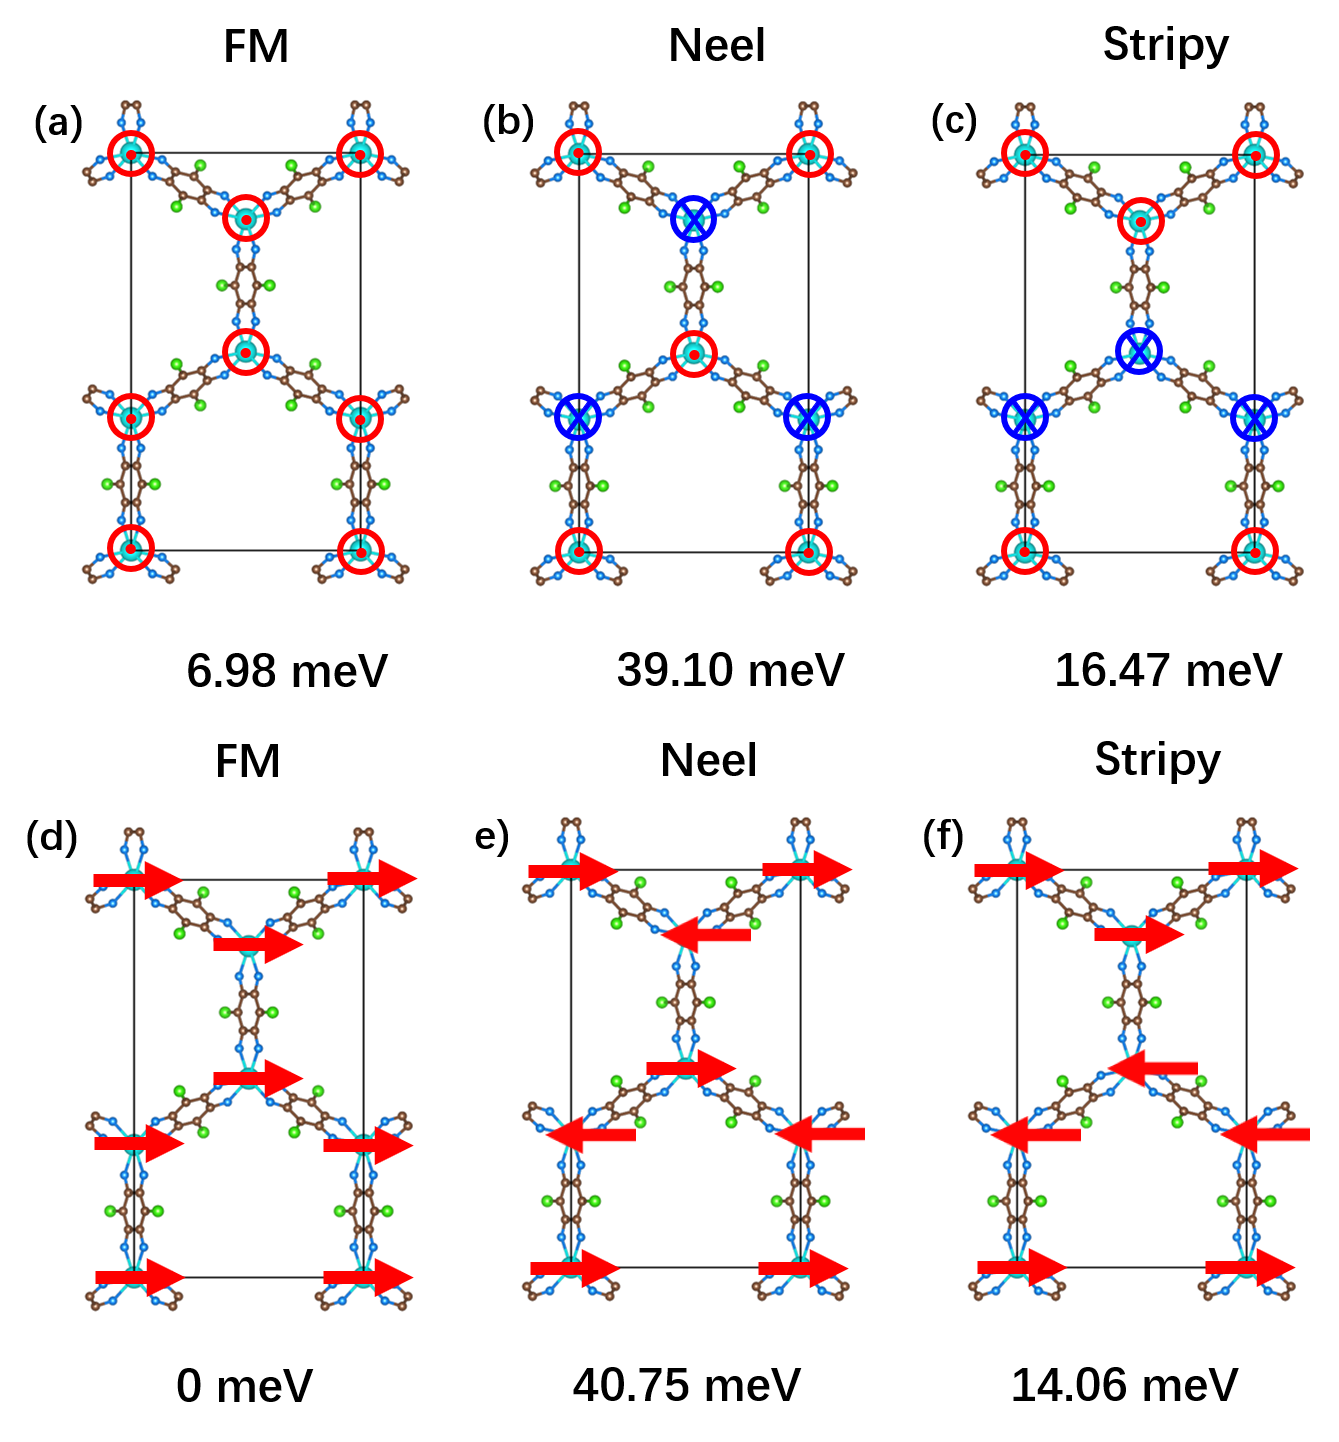
\includegraphics[width=0.5\textwidth]{PQAHEMagnetismAnisotropic.png}
  \caption{((a)Pr$_2$(C$_6$O$_4$Cl$_2$)结构的主视图和侧视图。2个Pr原子标记为I和II,周围6个圆圈为拟合的瓦尔尼有效轨道中心。(b)未考虑SOC自旋极化的能带。实线是DFT的
  结果,圆圈为瓦尼尔拟合的结果。(c)6个有效拟合的瓦尼尔轨道。红色和蓝色表示轨道不同的相位。}
  \label{PQAHEMagnetismAnisotropic}
  \note{}
\end{figure}

然后,我们计算了未考虑SOC的Pr$_2$(C$_6$O$_4$Cl$_2$)的能带结构,如图
\ref{PQAHEPrdhbqStrcture}(b) 所示。在费米面附近,发现单个自旋成分的Four 和 Dirac能带,跟我们之前提出的模型的能带(图\ref{PQAHEForeBand}(a)) 一样。为了直接建立这种
2维 MOF材料与我们提出的非线性轨道构成的2维 star 模型的联系,我们进行了瓦尼尔轨道拟合计算。如图\ref{PQAHEPrdhbqStrcture}(b)所示, 瓦尼尔拟合的能带(圆圈)几乎完全与
DFT计算的能带(实线)一致。拟合后的6个有效瓦尼尔轨道如图\ref{PQAHEPrdhbqStrcture}(c)所示。我们可以看到6个瓦尼尔轨道位于2个Pr原子附近(图\ref{PQAHEPrdhbqStrcture}(a)的圆圈)
形成2维的star晶格。此外,每个Pr原子附近的有效轨道(I和II两组)是相同,只是只是相对其它2个旋转了120度,分别形成顺时针和逆时针的涡旋取向。这些特征与我们前面提出的模型的特征
是一致的。

\begin{figure}[htb]
  \centering
  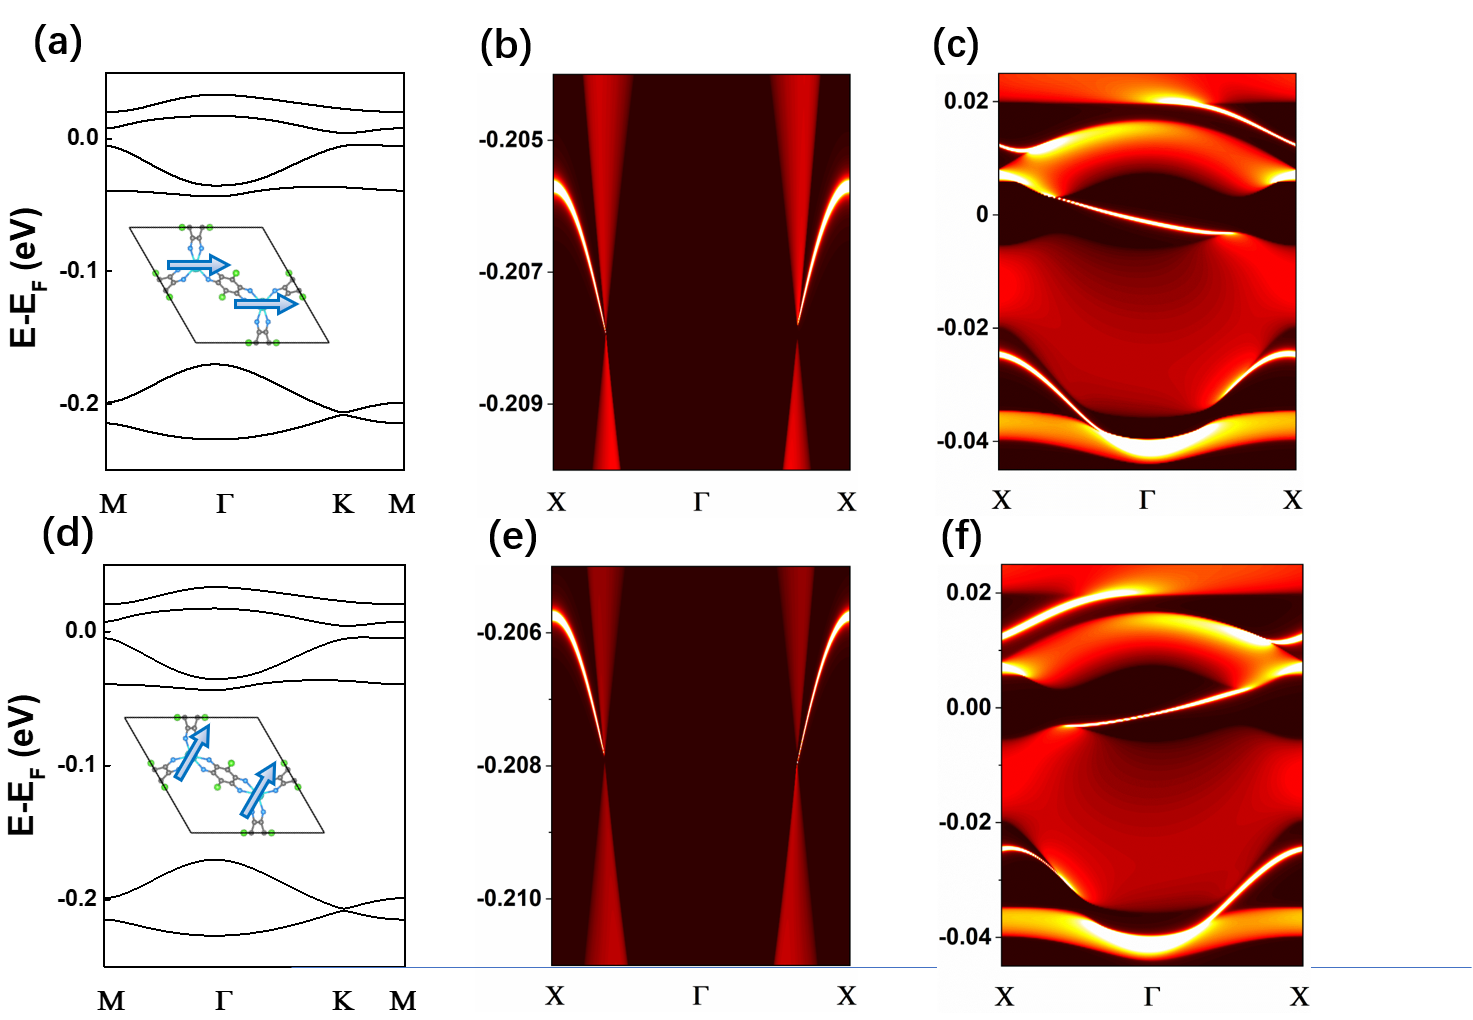
\includegraphics[width=0.9\textwidth]{PQAHEPrdhbqEdgeState.png}
  \caption{((a)考虑SOC后面内磁矩方向为0度时的能带。(b)和(c)磁矩方向为0度时的半无限普函数。(d-f) 与(a-c)一样,但磁矩方向为面内60度。}
  \label{PQAHEPrdhbqEdgeState}
  \note{}
\end{figure}

考虑SOC以后,面内磁矩方向为0度和60度时的能带结构分别如图\ref{PQAHEPrdhbqEdgeState}(a)和(d)所示。Dirac 和 Four 能带的兼并被SOC打开带隙,与我们提出的模型是一致的
(图\ref{PQAHETB30}(b))。为了检查能带的拓扑性质,我们分别计算了磁矩方向为0度和60度时的半无限普函数,如图\ref{PQAHEPrdhbqEdgeState}(b和c)和(e和f)。我们可以在图中看
到2个显著的特点。第一,在SOC打开的能隙中有一个1维的拓扑边界态。第二,图\ref{PQAHEPrdhbqEdgeState}(b和c)拓扑边界态展现陈数为-1的群速度,
而图\ref{PQAHEPrdhbqEdgeState}(e和f)拓扑边界态展现陈数为1的群速度,正好恰恰相反。改变面内磁矩的角度,这种拓扑边界态始终存在SOC带隙中,但是它的群速度却每隔60度改变一下
符号。也就是说,拥有 C = $\pm$1 PQAHE 被 $\alpha$ = $30 ^\circ$, $90 ^\circ$, $150 ^\circ$, $2100 ^\circ$, $270 ^\circ$ 和 $330 ^\circ$ 相变边界点所分隔。
因此在费米面附近, 我们可以获得一个周期性跳跃的量子化电导, 如图\ref{PQAHEQuantumConduction}(a)所示。
不同面内磁矩方向的相关的贝里曲率和陈数见图\ref{PQAHEQuantumConduction}(b)。 因此Pr$_2$(C$_6$O$_4$Cl$_2$)材料证明我们所提出的模型可行性,即在2维star 晶格中
非线性轨道可以产生的面内量子反常霍尔效应。

\begin{figure}[htb]
  \centering
  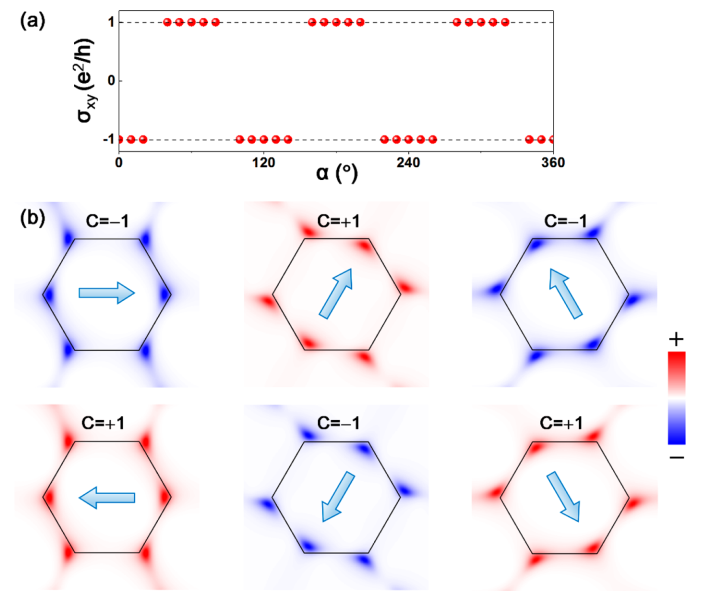
\includegraphics[width=0.9\textwidth]{PQAHEQuantumConduction.png}
  \caption{((a)Pr$_2$(C$_6$O$_4$Cl$_2$)不同面内磁矩方向下的量子化电导。(b)不同面内磁矩方向下的贝里曲率}
  \label{PQAHEQuantumConduction}
  \note{}
\end{figure}

\section{本章小结}
在本章中,我们提出一个由非线性轨道构成的2维star晶格紧束缚模型。通过模型的计算,我们发现这个模型可以打开同自旋下K点和$\Gamma$点的兼并能带的能隙,
从而实现面内量子反常霍尔效应。这完全不同于之前人们所提出实现面内量子反常霍尔效应的模型。
然后我们系统地研究不同$\theta$角度有效轨道和不同$\alpha$角度面内塞曼场下的相图,计算结果表明我们所提出的模型具有很高的可调性。
接着,我们找到一个实验上已经合成的金属有机框架材料Pr$_2$(C$_6$O$_4$Cl$_2$)。通过DFT和瓦尼尔拟合的计算,我们发现这个材料符合我们所提出的模型。
从而理论上第一次预言它是一个可以实现面内量子反常霍尔效应的金属有机框架材料。我们相信这种新型的面内量子反常霍尔效应可以很容易推广到其他有机金属框架材料中,
从而提供新的机会在未来去探索非线性轨道相关的拓扑物理学,拓宽相关的应用。